\scanpage{142}
\deleted{$\mathfrak m/\mathfrak m^2$}
\[
\begin{array}{ll}
\text{\unsure{espace} affine sous}&\unsure{\mathcal T|\mathcal J}^{0}_{B_0/A_0}\otimes V_1\\
\text{\unsure{espace} affine sous}&\unsure{\mathcal T|\mathcal J}^{0}_{B_0/A_0}\otimes V_2\\
&\unsure{\mathcal T|\mathcal J}^{0}_{B_0/A_0}\otimes V_3\qquad\unsure{\mathcal T|\mathcal J}_{V_0/}
\end{array}
\]
\figure{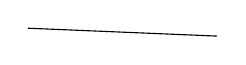
\begin{tikzpicture}\draw (0,0)--(2.4,-.1);\end{tikzpicture}}

$G_{A,n}=$ groupe algébrique sur $k$ des changements de \unsure{base} de la forme
\[
\left\{\begin{array}{l}
f_i=a_i+\displaystyle\sum_jb_{ij}t_j+\displaystyle\sum_{2\leq|p|\leq N}c_{ip}t^p\qquad a_i,b_{ij},c_{ip}\in A\\
a_i\in\mathfrak m,\ \det(b_{ij})\notin\mathfrak m
\end{array}\right.
\]

$G_n$ groupe sur $\mathbf Z$ des changements de \unsure{base}
\[
\left\{\begin{array}{l}
f_i=a_i+\displaystyle\sum\unsure{a_j|b_{ij}}t_j+\displaystyle\sum_{2\unsure{\leq|<}|p|\leq N}c_{ip}t_1^{p_1}\unsure{-|\ldots}t_n^{p_n}\\
\det(b_{ij})\ne0
\end{array}\right.
\]
i.e. les automorphismes de

\[
\deleted{\unsure{a+t}}\quad a_0+a_1t+a_2t^2
\]
\[
\deleted{a'_0+a'_1(a_0+a_1t)+\unsure{a'_2a_0^2}}
\]
\figure{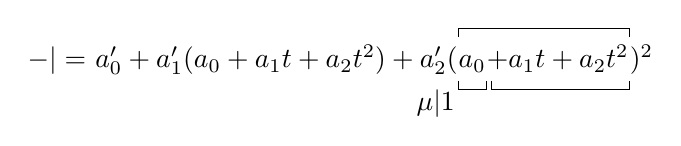
\begin{tikzpicture}[baseline=(prefix.base),inner sep=0pt]
\node[anchor=base west] (prefix) at (0,0) {$\unsure{-|=}\ a'_0+a'_1(a_0+a_1t+a_2t^2)+a'_2($};
\node[anchor=base west] (constant) at (prefix.base east) {$a_0$};
\node[anchor=base west] (tail) at (constant.base east) {$+a_1t+a_2t^2$};
\node[anchor=base west] at (tail.base east) {$)^2$};
\coordinate (upperleft) at (constant.west |- tail.north);
\coordinate (lowerleft) at (constant.west |- tail.south);
\coordinate (lowermid) at (constant.east |- tail.south);
\draw ([yshift=3pt]upperleft)--([yshift=6pt]upperleft)--([yshift=6pt]tail.north east)--([yshift=3pt]tail.north east);
\draw ([yshift=-3pt]lowerleft)--([yshift=-6pt]lowerleft)--([yshift=-6pt]lowermid)--([yshift=-3pt]lowermid);
\draw ([xshift=2pt,yshift=-3pt]tail.south west)--([xshift=2pt,yshift=-6pt]tail.south west)--([yshift=-6pt]tail.south east)--([yshift=-3pt]tail.south east);
\node[anchor=north east] at ([xshift=-1pt,yshift=-6pt]lowerleft) {$\unsure{\mu|1}$};
\end{tikzpicture}}
\[
k[t]/(t^3)\qquad
\boxed{\begin{aligned}
={}&(a'_0+a'_1a_0+a'_2a_0^2)\\
&+(a'_1a_1+\unsure{2|[}a'_2a_0a_1)t\\
&+(a'_1a_2+a'_2a_1^2+2a'_2a_0a_2)t^2
\end{aligned}}
\]
\[
\phantom{=}+2a'_2a_1a_2t^3
\qquad +a'_2a_2^2t^4
\]
\margin{141}
